

\documentclass{sig-alternative}
\usepackage{multirow}
\usepackage{color}
\usepackage{graphics}
\usepackage{rotating}
\usepackage{graphics}
\usepackage{colortbl} 
\usepackage{picture}
\usepackage{algorithm}
\usepackage{algorithmicx}
\usepackage{algpseudocode}
\definecolor{lightgray}{gray}{0.8}
\definecolor{darkgray}{gray}{0.6}
\renewcommand{\algorithmicrequire}{\textbf{Input:}}
\renewcommand{\algorithmicensure}{\textbf{Output:}}
%%% graph
\newcommand{\crule}[3][darkgray]{\textcolor{#1}{\rule{#2}{#3}}}
\newcommand{\rone}{\crule{1mm}{1.95mm}}
\newcommand{\rtwo}{\crule{1mm}{1.95mm}\hspace{0.3pt}\crule{1mm}{1.95mm}}
\newcommand{\rthree}{\crule{1mm}{1.95mm}\hspace{0.3pt}\crule{1mm}{1.95mm}\hspace{0.3pt}\crule{1mm}{1.95mm}}
\newcommand{\rfour}{\crule{1mm}{1.95mm}\hspace{0.3pt}\crule{1mm}{1.95mm}\hspace{0.3pt}\crule{1mm}{1.95mm}\hspace{0.3pt}\crule{1mm}{1.95mm}} 
\newcommand{\rfive}{\crule{1mm}{1.95mm}\hspace{0.3pt}\crule{1mm}{1.95mm}\hspace{0.3pt}\crule{1mm}{1.95mm}\hspace{0.3pt}\crule{1mm}{1.95mm}}
\newcommand{\quart}[3]{\begin{picture}(100,6)%1
{\color{black}\put(#3,3){\circle*{4}}\put(#1,3){\line(1,0){#2}}}\end{picture}}
\definecolor{Gray}{gray}{0.95}
\definecolor{LightGray}{gray}{0.975}

%% timm tricks
\newcommand{\bi}{\begin{itemize}[leftmargin=0.4cm]}
\newcommand{\ei}{\end{itemize}}
\newcommand{\be}{\begin{enumerate}}
\newcommand{\ee}{\end{enumerate}}
\newcommand{\tion}[1]{\S\ref{sect:#1}}
\newcommand{\fig}[1]{Figure~\ref{fig:#1}}
\newcommand{\eq}[1]{Equation~\ref{eq:#1}}

%% space saving measures

\usepackage[shortlabels]{enumitem} 
\usepackage{times}

\usepackage{url}
\def\baselinestretch{1}


\setlist{nosep}
 \usepackage[font={small}]{caption, subfig}
\setlength{\abovecaptionskip}{1ex}
 \setlength{\belowcaptionskip}{1ex}

 \setlength{\floatsep}{1ex}
 \setlength{\textfloatsep}{1ex}
 \newcommand{\subparagraph}{}

\usepackage[compact,small]{titlesec}
\DeclareMathSizes{7}{7}{7}{7} 
\pagenumbering{arabic}
\setlength{\columnsep}{7mm}

\begin{document}

\conferenceinfo{FSE}{'15 Bergamo, Italy}
\title{Implications of Differential Evolution for  Defect Prediction:
Analytics Without Parameter Tuning Considered Harmful}
\numberofauthors{1}
\author{
\alignauthor
Wei Fu, Tim Menzies\\
       \affaddr{Computer Science, North Carolina State University, USA}\\
       {wfu@ncsu.edu, tim.menzies@gmail.com}} 


 
\maketitle
\begin{abstract}


software defect prediction with various 
empirical data sets. Those proposed leaners are always evaluated against the state of the art 
predictors by performing statistical analysis. Undoubtedly, given the bias from data sets and 
accuracy indicators, the newer predictors outperform counterparts in selected experimental 
settings. However,  most of data mining algorithm based predictors (e.g. CART, random 
forest, 
neural networks, SVM) have built-in {\it magic} parameters, like the number of trees in random 
forest algorithm. the impact of internal parameters in those methods have been neglected 
during evaluation. In this paper, we investigate this impact by tuning parameters in defect 
predictors with search-based software engineering algorithm. Specifically, we used differential 
evolution to tune the CART and a new predictor based on WHERE algorithm with local data, 
and then predictors with optimal parameters obtained from tuning process will be applied to 
predict defects. By comparing the performance of predictors with and without tuning process,  
we observe that tuning improves the predictors' performance and predictors woking with 
different data sets need different parameters. Our results also suggest that we should not use 
the predictors of the shelf with their default parameters and tuning should be a processor 
combined with any predictor with built-in parameters.


%RQ1: Does tuning affect learners' performance?
%RQ2: How to choose 

\end{abstract}

% A category with the (minimum) three required fields
\vspace{1mm}
\noindent
{\bf Categories/Subject Descriptors:} 
D.2.8 [Software Engineering]: Product metrics;
I.2.6 [Artificial Intelligence]: Induction

\vspace{1mm}
\noindent
{\bf General Terms:} Experimentation, Algorithm

\vspace{1mm}
\noindent
{\bf Keywords:} defect prediction, CART, random forests,
Fastmap,   bootstrap sampling, effect size, A12.

\section{Introduction}

\begin{raggedleft}
{\em ``The  common misunderstanding about science 
is that scientists seek and find truth. They don't- 
they make and test models.''}\\ -- Neil Gershenfeld

{\em Essentially, all models are wrong, but some are useful."}\\ --George Box

\end{raggedleft}

XXX One consequence of this work is that it is possible to tune a detector such that it exhibits a wide range of performance scores. Given that, the next question becomes ``what performance scores do you want?''. This is an interesting issue since there is no single best answer. XXX

How ``true'' are the  models generated by software analytics?
Suppose we use a model generated from software project data to, for example,
assess the relative value of OO metrics vs procedural metrics for predicting
project defects. Are we reporting ``truth'' in any sense of the word? And for how
many other projects  and how many kinds of questions might we find that same ``truth''? 

This is not some abstract question-- it is an open and pressing matter.
Any reading of the recent proceedings of FSE, ICSE, ASE, etc will discover hundreds
of papers using data miners to make conclusions about software projects. 
For example, some  analysts have made conclusions
about 
{\em what attributes
have most influence on a software project}.
For example, in 2013,
Rahman et al
\cite{rahman2013how}  used results from logistic regression to conclude
that code metrics are generally less useful than process
metrics for  predicting defects from static code analysis.  
In the same year, Bell et al. (who also used negative binomial regression) argued that
software defect prediction was not improved by adding in~\cite{bell2013limited}.

@article{bell2013limited,
  title={The limited impact of individual developer data on software defect prediction},
  author={Bell, Robert M and Ostrand, Thomas J and Weyuker, Elaine J},
  journal={Empirical Software Engineering},
  volume={18},
  number={3},
  pages={478--505},
  year={2013},
  publisher={Springer}
}

The results of this paper offer a very different picture  to recent prominent results from prior authors.
Lessmann et al.~\cite{lessmann2008benchmarking}, Rahman et al.~\cite{rahman2013how} and Arshiholm et al.~\cite{arisholm06} argue that when it comes to defect prediction, different learners often
produce statistically similar results. For this reason  Rahman et al. only present results their logistic
regression results, commenting that ``dor brevity, only results from LR are
presented; other learning models give similar results''~\cite{rahman2013how}. Note that those prior results,
where most learners achieved the same results, arose from the default parameter settings from those learners.

Our results, on the other hand, come from tuning a data miner's parameters. In those results,
we found that the choice of parameters had dramatic impacts on data mining performance.
For example, we show results below where:   
\bi 
\item 
Tuning improved precision values from  2\% to 98\%; or
\item 
Tuning improved false alarm values from 69\% to 0\%; or
\item 
Tuning improved recall values from 0 to 100\%; or
\item 
Tuning improved the f-measure (which is the harmonic mean of recall and precision) from 0 to 86\%.
\ei   
In terms of changing SE research methodologies, an important aspect of these results is that usually XXXX always different. cannot determine without experimentation which learner will, after tuning, yield the best results for a particular data set. Hence it is no longer viable for researchers to trust the recommendations 
of other researchers working with other data sets that ``data miner XYZ is best''. Before
offering a conclusion about a particular data set, researchers need now augment  their 
papers with preliminary tuning studies (the results of which select the tunings+data miners to be used
to make conclusions for the second half of their paper).

The good news is that such tuning is not an arduous task. The differential evolution algorithm 
used in this study is wdiely available in many standard  toolkits and languages\footnote{See the long list at
www1.icsi.berkeley.edu/~storn/code.html.}
And even if somehow those tools and prior implementations are not workable at a local site, 
differential evolution is very simple to code. Hence, it can readily and quickly implemented.
 

When we discuss these results with colleagues, one response we get is ``enough of the parameter tuning.. lets use simpler methods''. 
While we understand their motivation (to keep thing simple), software project
data cannot necessarily be condensed to (say) a simple univariate analysis that
reports how one independent variable effects a dependent variable.
Such a simplistic analysis can miss significant interaction
effects when multiple factors combine to effect the target variable. For example,
one of the base results in defect prediction is that predictors formed from
a single variable perform much worse than those can combined multiple variables (three or more)~\cite{me07b}.

If those results come from an analysis of a complex interactions between attributes,
then some kind of data mining method\footnote{By this term we mean the
full gamut of methods for large-scale analysis of
data including statistical
parametric methods (that assume a particular distribution then strive to learn the parameters of that distribution); kernel methods;
dimensionality  synthesis methods; 
instance weighting schemes; feature subset selection methods
outlier removal methods;
decision tree learners; neural networks; and instance-based
methods including clustering and/or   case-based reasoning.} then there is the
{\em tuning problem} of how to set the myriad of parameters that 
control the learner.

\item
What data miners are better than others for particular tasks
in software analytics. 
\ei



Also, in 2007, one of us (Menzies) claimed that Naive Bayes
classifiers with a certain lind of pre-processor were better than entropy-based decision trees for defect prediction~\cite{me07b}.
Similarly, in 2008 Lessmann et al.~\cite{lessmann2008benchmarking} argued  that 
Random Forests~\cite{brieman00} and CART ~\cite{brieman84} work best, worst for learning software defect predictors from
static code attributes. Similar claims that one learner was better than another
have been made by many other authors; e.g. 
 
 


We write to suggest that all those conclusions may be wrong or, at the very most,
correct within a very limited context. At the very least, the conclusions
of those papers (and literally dozens of similar papers, include severl
of our own~\cite{me02e,me02k,me03a,me06d,me07b}) need to be revisited
in light of this paper's results on the effects of tuning on data miners.

Machine learners
are controlled by parameters that decide (e.g.) when to stop recursively
dividing data into smaller section or (e.g.) what thresholds for errors are small
enough to be acceptable. When used ``off-the-shelf'', analytst
use default settings for those parameters. We find that  a 
simple optimization scheme (differential evolution) can find much
better tunings that can dramatically change the performance of
the learned model (measured in terms of false alarm rates, recall,
precision, f-measure, and g-measure).  From this first result,
we conclude that {\bf parameter tuning with some optimizer such as differential
evolution should become standard practice}.

Our next observation is that observations about miner1 being better
than miner2 do not survive tuning. To be specific: given some
ranking of data miners for some task such as defect prediction,
we find that tuning can reverse those rankings such that the worst untu


Tuning the data miners with different evolution takes some
times (around an order of magnitude slower than the learning), but not an impractically slower amount of time. Further, when we look at what
attrub


Our reading of the 

good news:
\bi 
\item Tuning is easy (but one measure, at least an order of magnitude easier than 
standard optimization problems)
\item Tuning can dramatically improve the performance of a learner (in one case, from recalls
of zero to 70\%)
\ei
interesting news
\bi 
\item tunings different for different data sets.
\ei 
bad news:
\bi
\item Tuning also changes what was learned
\bi
\item Supposedly ``bad'' learners start working much better than supposedly ``best'' learners;
\item The models used in the tuned models were very different to those used in the untuned learners.
\ei 
\ei 
and we reflect on that model, are we 

will it reveal the `1`t
A standard approach to software analutics
Software has becoming a large and complex system and delivering reliable and quality 
software is imperative for development teams. Empirical study shows that the longer the 
defects exist in software systems, the more the cost of time and money it will take to fix it 
\textbf{ [need a ref]}. Therefore, project managers and software programers strive to find 
defects in their system as early as possible. Defect prediction has been investigated 
extensively in industrial and academia during the past two decades. As an important research 
field, building data miners  \cite{lessmann2008benchmarking, mccabe1976complexity, 
menzies2007data, menzies2010defect, jiang2008can, menzies2011local, song2011general} 
over static code features of software system has been demonstrated to be a way to predict 
which models are more likely to contain defects.

Classification is an important approach to predict whether some modules in the projects are 
defective or non-defective. The general idea is to train the learners by using parts of data 
sets(e.g. ant 1.3, 1.4 in PROMISE\footnote{http://openscience.us/repo/}) and predict with 
remaining ones(ant 1.5, 1.6 and 1.7). Many types of defect predictors have been proposed 
based an different data mining classifiers, including CART, Random Forest 
\cite{guo2004robust},  Naive Bayes\cite{menzies2007data},Logistic Regression 
\cite{khoshgoftaar1999logistic}. During the past years, authors claimed that their new 
defective learner outperformed others according to their experiment and statistical analysis. 
To evalute those learners objectively in terms of accuracy, Lessmann et al
\cite{lessmann2008benchmarking} carried out a study to compare 22 classifiers over 10 public 
\begin{figure}
\small
\begin{tabular}{|p{.95\linewidth}|}\hline
When applying case-based reasoning, researchers use different settings including how they measure dis- tance between instances (examples include the Euclidean measure, Manhattan and Chebyshev). Other settings control if numerics are normalized min..max to 0..1, before they are used in the distance measure.

Another set of settings refers to how to handle non-numeric distances or missing values. Some researchers delete training data with missing information while others compute missing values via, say, median values.

After feature selection comes instance selection. There are many settings for instance selectors such as use outlier removal or prototype generation. Within each of those settings are number sub-choices such as the choice of outlier remover or prototype generator.
The next set of settings concern how many neighbors to use (k=1,2,5,etc). Some researchers set ``k'' in dynamic pre-learning phase that checks the training data to find what ``k'' works best for that data.

Once the neighbors are known, the next settings control how to summarize their information. Some researchers use means, other use medians, or a weighted sum that uses the distance of the neighbor from the test instance (and that weighting might be determined by some kernel such as uniform, triangular, Gaussian, cosine, or Epanechnikov).
Researchers may use other settings to control different pre-processors. E.g. some discretize numeric values (via equal width or equal frequency) using some binning policy (and researchers differ on how many bins are best).\\\hline
\end{tabular}
\caption{Some tunings for SE predictive systems. Found by this author while preparing this proposal in a day of reading the SE predictive modeling literature on case-based reasoning and effort estimation. Note that other kinds of prediction systems (decision trees, neural nets, linear repression, etc) have yet more adjustable design options.}\label{fig:adjust}
\end{figure}

domain data sets from the NASA Metrics Data repository. By using Nemenyi's post hoc test 
with $\alpha = 0.05$, they concluded that the predictive accuracy of most learners didn't differ 
significantly in terms of the area under the receiver operating characteristics curve(AUC). 
Furthermore, according to the fig.2 in \cite{lessmann2008benchmarking}, Random Forest is 
significantly better than CART. Lessmann's paper motivates us to investigate whether tuning 
those CART's parameters by search-based software engineering method can improve the 
performance. Even though Lessmann considered unpruned tree and pruned tree, They didn't 
consider other possible parameters in CART which would have impact on the structure of 
trees, like the depth of the tree, the maximum and minimum number of leafs of the tree.

Software metrics are the core of all the defective prediction model. Many types of metics
are used to build models, like process metrics, McCabe and Halsted metrics  and CK metrics.
By building prediction modes across 85 releases of 12 open source projects, Rahman et al
\cite{rahman2013how}  concluded that code metrics are generally less useful than process
metrics for prediction. And also the code metrics don't change much from release to release
and lead to stagnation in the prediction model. In \cite{Radjenovi?20131397}, Radjenovi? et al
\cite{Radjenovi?20131397} reviewed 106 papers regarding software prediction metrics. They found
that CK objected-oriented and process metrics have been reported to be more successful in
finding defects compared to traditional size and complexity metrics. Moreover, not all the CK
metrics perform well equally. The best metrics from CK are CBO, WMC and RFC based on their 
observation. It seems that the relationship between software metrics and defective prediction is
still an open question and need to be addressed. This motivates us to see : whether the impact
rankings of those metrics will change after tuning parameters
is applied to model learners.



What's the problem in those result?

RQ:

briefly describe our study and  our result; observation

structure of this paper.

\subsection{Implications}

time for an end to era of data mining in se? moving on to a new phase of learning-as-optimization

1) learning is actually an optimization tasks (e.g. see fig2 of  learners climbing the roc curve hill in http://goo.gl/x2EaAm)

2) our learners are all contorted to do some tasks X (e.g. minimize expected value of entropy), then we assess them on score Y (recall). which is nuts. maybe we should build the goal predicate into the learner (e.g http://menzies.us/pdf/10which.pdf) 

3) given 1 + 2, maybe the whole paradigm of optimizing param selection is wrong. maybe what we need is a library of bees buzzing around making random choices (e.g. about descritziation) which other bees use, plus their own random choices (e.g. max depth of tree learned from discretized data) which is used by other bees, plus their own random choices (e.g. business users reading the models).  the funky thing here is that it can take some time before some of the bees (the discretizers) get feedback from the community of people using their decision (the tree learners). 

\section{Algorithm: Predictor and Tuner}

In order to conduct the experiment of this paper, we need one tool that can predict defects 
from the empirical data sets and a second tool to tune the built-in parameters associated with 
predictor. To compare the effects of the tuning process, we have three different predictors: 
WHERE-based Predictor, CART and Random Forest. Different Evolution(DE) as an optimizer 
is used as a tuner in this paper.

We choose CART and Random Forest as a predictor in this paper is motivated by 
\cite{lessmann2008benchmarking}, where the performance of both tools as predictors are 
significantly different based on authors' experiment as mentioned before. We'd like to 
investigate whether tuning can change such conclusion. WHERE-based Predictor is a new 
defect predictor based on WHERE\cite{menzies2013local} algorithm. A comparison with 
standard predictor like CART and Random Forest will better evaluate and judge the 
performance such new predictor. As for the tuner, there're many heuristic optimization 
algorithms in wild. However, DE is a good but maybe not the best candidate for the tuning 
process considering different performance measurements. To determine which optimizer is 
fitable and results in better performance is beyond this work scope. We leave it to future 
works. The rest of this section will describe each tool applied in this work.

 \subsection{WHERE-based Learner}
\textbf{WHERE-based Learner} is composed of WHERE clustering algorithm and CART 
decision tree algorithm. The key idea of WHERE-based learner is that  instead of training the 
CART decision tree based on the class labels associated with each training sample, it's using 
CART to build decision trees based on the cluster labels, which are generated by the WHERE 
clustering algorithm.
 
 
 
\begin{figure}[!t]

\renewcommand{\baselinestretch}{0.8}
\scriptsize
\centering
  \begin{tabular}{r@{~}|r@{~}rr|r@{~}rr|r@{~}rr}
    & \multicolumn{3}{c|}{WHERE}&\multicolumn{3}{c|}{CART}& \multicolumn{3}{c}{Random Forest}\\\cline{2-10} 
    Goal & tuned & naive &$\frac{\mathit{tuned}}{\mathit{naive}}$& tuned & naive &$\frac{\mathit{tuned}}{\mathit{naive}}$& tuned & naive&$\frac{\mathit{tuned}}{\mathit{naive}}$\\\hline
pd&71.4&1.2&60&4.4&0.1&44&7.1&0.2&36\\ 
prec&82.8&1.4&59&3.9&0.1&39&7.4&0.2&37\\
f&86.1&1.2&72&3.3&0.1&33&6.7&0.2&34
  \end{tabular}
  \caption{For one train/test set pair (ANT),  time (in seconds) spent tuning,
  for different goals, or just running the ``off-the-shelf'' learner.}
\end{figure}


\begin{figure}[!t]

\renewcommand{\baselinestretch}{0.8}
\scriptsize
\centering
\begin{tabular}{r|rrr}
goal &	WHERE	&CART&	Random Forest\\\hline
f	&15	&13	&9\\ 
pd	&15	&16	&8\\ 
prec&	14	&14	&8
\end{tabular}
\caption{How much slower is tuning vs just running the default
settings of the learner? E.g. bottom right, tuning to increase
precision with Random Forests is eight times slower than
just running Random Forests.}
\end{figure}



% Given N instances, instead of building decision tree directly with CART, we use WHERE to 
%cluster instances. 
WHERE is a fast clustering algorithm designed by {\it menzies} for finding software artifacts 
with similar attributes. It clusters data on dimensions synthesized along the axis of greatest 
variability in the data. The way WHERE used to find such dimension is a linear-time heuristic 
called ``FASTMAP" proposed by Faloutsos \& Lin\cite{faloutsos1995fastmap}. ``FASTMAP" 
randomly picks one instance $Z$; find the instance {\it east} $X$ that's furthest away form $Z$; find 
the instance {\it west} $Y$ that's furthest away from {\it east} $X$. Next, project all the remaining 
points onto the line drawn between $X$ and $Y$.  The line $\overline{XY}$ is an approximation of the 
first component found by PCA. As shown in Figure \ref{Where}, $X$ and $Y$ are the furthest points found by ``FASTMAP'' and $\overline{XY}$ is of length $c$. Each point in this figure has a distance $a$
to $X$ and distance $b$ to $Y$. According to the coisne rule and Pythagoras, each instance will be mapped 
into 2-dimension by the following equations.
\begin{equation}
	\begin{split}
			x  &= (a^2 +c^2-b^2)/(2c)\\ 
		    y  &= \sqrt{a^2 -x^2}
	\end{split}
\end{equation}


Then choose the median point $\hat{x}$ as the split and 
recursively divide all the instances into {\it west} and {\it east} clusters until the number of 
instances within each cluster is less than specific minimum size. The representation of the 
clustering result is a tree, we call it Where-clustering tree. Such tree will be pruned if applicable 
in some cases. Finally, cluster labels  will be assigned to instances in each of those 
clusters(leaves). 

\begin{figure}[!ht]
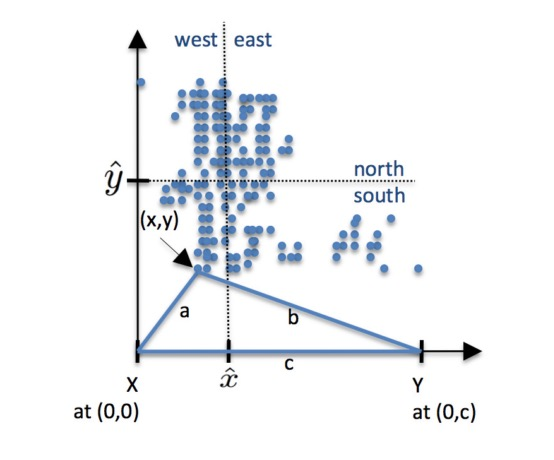
\includegraphics[scale=0.5]{where.png}
\caption{WHERE algoirthm }
\label{Where}
\end{figure}
Then based on the attributes and the cluster labels in each instances,  we build a 
decision tree based on CART algorithm. In each leaf of the tree, there're several instances 
falling in. This will be the model trained for defect prediction. During testing process, a new 
instance comes in and traverses the tree according to 
values of the its attributes. If the instance could reach one leaf of the tree, the predicted value 
of this instance will be the mean  of all the training data values associated with this leaf. 
Otherwise if stops at intermediate nodes of tree, the predicted value will be the mean of the all 
the training data value below this node. After estimating all the number of defectives in the test 
data, whether each instance contains defectives will be determined by comparing with a threshold value. If the predicted value is greater than threshold, the Where-based learner will predict this instance as defective otherwise non-defective.


%\begin{algorithm}
%	\caption{Pesudocode for WHERE Algorithm }
%	\label{alg:WHERE}
%		\begin{algorithmic}[1]
%			\Require $data$
%			\Ensure $tree$
%		\Function {Fastmap}{$ data$}
%			\State $one \gets$ any$(data)$
%			\State $west \gets$ furthest$(data, one)$
%			\State $east \gets$ furthest$(data, west)$
%			\State $c \gets$ distance($west, east$)
%		\EndFunction
%	 \end{algorithmic}            
%\end{algorithm}

\subsection{CART}
\textbf{CART} is an {\em iterative dichotomization} algorithm
that finds the attribute that most divides the data such that
the variance of the goal variable in each division is
minimized\cite{breiman84}.
The algorithm then recurses on each division.
Finally, the cost data in the leaf divisions
is averaged to generate the estimate.

\subsection{Random Forests}

Breiman's website describes \textbf{Random Forests} as
follows\cite{brieman00}. "Random Forests grows many classification
trees. To classify a new object from an input vector, put the input
vector down each of the trees in the forest. Each tree gives a
classification, and we say the tree "votes" for that class. The forest
chooses the classification having the most votes (over all the trees
in the forest). Each tree is grown as follows.
If the number of cases in the training set is N, sample N cases at
random - but with replacement, from the original data. This sample
will be the training set for growing the tree.
Also, if there are M input variables, a number m$<<$M is specified such
that at each node, m variables are selected at random out of the M and
the best split on these m is used to split the node. The value of m is
held constant during the forest growing.
Finally, each tree is grown to the largest extent possible (there is
no pruning)."




%Suppose the cordinates of X and Y are $(0,0)$ and $(0,c)$, which are east and west 
%instances within N samples. From the Pythegoras and cosine rule, each instance is projected 
%at the point(x,y)
%
%\begin{equation}
%	\begin{split}
%	x &= (a^2 + c^2 - b^2)/(2c) \\
%	y &= \sqrt{a^2 - x^2} 
%	\end{split}
%\end{equation}




\subsection{Differential Evolution Algorithm}
Differential Evolution (DE)\cite{storn1997differential} is a stochastic search algorithm that 
optimizes a problem by iteratively trying to improve a  population of candidate solutions with 
regard to a given quality measurement. Such method makes no assumptions about the 
problem being optimized and has already been used as a parameter tuner
\cite{omran2005differential, chiha2012tuning}.

DE starts with creating a population of candidate solutions and then generates new 
candidates based on $New = X+f*(Y-Z)$, where $X$, $Y$ and $Z$ are randomly selected 
solutions from the current frontier and $f$ is a crossover factor. The newly generated solution 
will be added into the next generation of solutions if dominating previous old points in the 
frontier. To avoid meaning less iteration, early termination strategy is applied that is at the 
beginning, assign a value to the $life$ parameter, it would be reduced by one each time   
when the new generation of candidate solutions does not improve in terms of quality 
measurement. The DE will stop when the $life$ equals to 0.

Algorithm \ref{alg:DE} is a list of pseudocode of DE with early termination for maximizing a 
score function, where $np$ is the number of population in each generation, $f$ is the 
crossover factor as mentioned, $cf$ is the probability for crossover operation to generate new 
candidate, $life$ is to control termination.

\begin{algorithm}
	\caption{Pesudocode for DE with Early Termination}
	\label{alg:DE}
		\begin{algorithmic}[1]
			\Require $np = 10$, $f=0.75$, $cr=0.3$, $life = 5$
			\Ensure $S_{best}$
	      
	      \Function{DE}{$np$, $f$, $cr$, $life$}
		  \State $Population  \gets $ InitializePopulation($np$)
		  \State $S_{best} \gets $GetBestSolution($Population $)
		  \While{$life > 0$}
			\State $NewGeneration \gets \emptyset$
			\For{$i=0 \to np-1$}
				\State $S_i \gets$ GenNew($Population [i], Population , cr, f$)
				\If {Score($S_i$) >Score($Population [i]$)}
				 	\State $NewGeneration$.append($S_i$)
				\Else
					\State $NewGeneration$.append($Population [i]$)
				\EndIf
			\EndFor
			\State $Population  \gets NewGeneration$
			\If{$\neg$ Improve($Population $)}
				\State $life -=1$
			\EndIf
			\State $S_{best} \gets$ GetBestSolution($Population $)
		  \EndWhile
		 \State \Return $S_{best}$
		 \EndFunction
		 \Function{Score}{$Candidate$}
		    \State set tuned parameters according to $Candidate$
		    \State TrainLearner()
		    \State $scores \gets$TestLearner()
		    \State \% scocres = [pd, f, precision]
		    \State $s \gets scores[i] $ 
		    \State \% i determines the goal of tuning
		    \State \Return$s$
		 \EndFunction
		 \Function{GenNew}{$old, pop, cr, f$}
		   \State $a, b, c\gets threeOthers(pop,old)$ 
		   \State \% pick 3 other points from the population
		   \State $newf \gets \emptyset$
		   \For{$i=0 \to np-1$}
		        \If{$cr < random()$}
		          \State $newf$.append($old[i]$)
                \Else
                  \If{typeof(old[i]) == bool}
                    \State $newf$.append(not $old[i]$)
		          \Else
		           \State $newf$.append(trim($i$,($a[i] + f * (b[i] - c[i]$))))
		           \State \%trim() will make new value fall in the range
		          \EndIf
		        \EndIf
		   \EndFor
		 \EndFunction
        \end{algorithmic}            
\end{algorithm}

%\begin{algorithm}
%\begin{algorithmic}[1]
% \KwData{this text}
% \KwResult{how to write algorithm with \LaTeX2e }
% initialization\;
% \While{not at end of this document}{
%  read current\;
%  \eIf{understand}{
%   go to next section\;
%   current section becomes this one\;
%   }{
%   go back to the beginning of current section\;
%  }
% }
% \caption{How to write algorithms}
% \end{algorithmic}
%\end{algorithm}

\section{Experiment}

\subsection{Data Set}

The data used in this study is from PROMISE repository. Ten software defect predicition data 
sets are analyzed. They're {\it ant}, {\it camel}, {\it ivy}, {\it jedit}, {\it log4j}, {\it lucene}, {\it 
synapse}, {\it velocity}, {\it xalan} and {\it xerces}. Each of these data sets is composed of 
several software modules with number of defects and code attributes. For more detailed 
description of code attributes and the original data sets, please refer to  http://openscience.us/
repo/

\subsection{Experiment Design}

The experiment aims at investigate whether tuning helps learners improve performance in 
terms of accuracy measurement. We choose compare WHERE-based learner with and 
without tuning parameters and two {\it significantly different} learners Random Forest and 
CART according to \cite{lessmann2008benchmarking}. As mentioned above, we'd like to see 
whether tuning will help change the rank of CART and make it comparable with Random 
Forest. 

To evaluate accuracy performance of learners, several measurements are proposed, like 
probability of  detection({\it pd}) and probability of false alarm ({\it pf})\cite{menzies2007data}, 
the area under the receiver operating characteristics curve ({\it AUC})
\cite{lessmann2008benchmarking}, and precision\cite{zhang2007comments}. In this work, we 
expect learners should identify as many defective modules as possible while avoiding false 
alarm. Therefore, learners are evaluated by both of {\it pd} and {\it pf} simaltanieously. A single 
measure, G-measure, defined as the harmonic mean of {\it pd} and $1-{\it pf}$  is used. The 
G-measure value is between 0 and 1. The higher, the better.
\begin{equation}
G = \frac{2*(1-pf)*pd}{1-pf+pd}
\end{equation}

In this experiment, we use three different portions of one project data set for training, tuning 
and testing process. In contrast to hold out way used in \cite{lessmann2008benchmarking, 
menzies2007data}, we separate the data sets in order. Since learners are designed to predict 
defects in future projects,  any randomly data set selection without taking into the time series 
will not sufficient to evaluate the performance of predicting future. To the most, that is good to 
evaluate the accuracy of classification but not predicting future. Since we have 10 different 
project data, each of which contains least 3 evolutionary versions. We use the following policy 
to select the data: in each project, we only use the last three data files for experiment. 
Specifically, the $nth$,  $(n-1)th$, $(n-2)th$ versions of project data are selected for testing, 
tuning and training learners, respectively. This will make sure that we don't use the future 
project data to train learners and predict previous project.

To investigates the impacts of parameters on learners, we use DE as the tuner and compare the G-measure 
values of Where-based learner with and without tuning, CART with and without tuning and Random 
Forests. Since the tuning time for Random Forests is very long, hopefully other researchers design
new heuristics to speed up the tuning process for Random Forests.  For the time being, even though
we don't tune Random Forests, if tuning help CART outperform Random Forests or improve itself performance ,
we still could conclude that tuning is helpful and necessary when comparing learners.

Besides the Where-based learner implemented by ourself,  we use the CART and Random Forest modules 
from scikit-learn \cite{scikit-learn} for this experiment. The parameters associated with different learners are listed in Fig.\ref{fig:parameters}. (\textbf{NEED to elaborate that there're different versions of CART, what's the point to do this experiment}). For each data set, run CART, naive Where-based learner and Random Forests with corresponding default values. Then using DE to tune corresponding parameters for CART and Where-based Learner,  and run them again with the optimal parameters from tuning process to test the performance. 
This study ranks learners using the Scott-Knott procedure recommended by Mittas \& Angelis in their 2013
IEEE TSE paper~\cite{mittas2013ranking}.  This method sorts a list of $l$ treatments with $ls$ measurements by their median score. It then splits $l$ into sub-lists $m,n$ in order to maximize the expected value of differences  in the observed performances before and after divisions. 

\section{Result}

\section{Discussion}

\section{Related Work}

Tuning in efforts estimation, software engineering.

Defect Prediction



\section{Threats to Validity}

Internal and external threats

\section{Conclusion}

\section{Acknowledgments}

\bibliographystyle{unsrt}
\bibliography{tuningpredictor}  




%%%%%%%%%%%%%%%% list of parameters%%%%%%%%%%%%%%%%%%%%%
\renewcommand\arraystretch{1.2}
\begin{figure*}[t!]
\renewcommand{\baselinestretch}{0.8}
\scriptsize
  \centering
	\begin{tabular}{|c|c|c|c|l|}
	\cline{1-5}
	\begin{tabular}[c]{@{}c@{}}Learner \\ Name\end{tabular} & Parameters & Default &\begin{tabular}[c]{@{}c@{}}Tuning\\ Range\end{tabular}& 
\multicolumn{1}{c|}{Description} \\ \hline
	\multirow{8}{*}{\begin{tabular}[c]{@{}c@{}}Where-based\\ Learner\end{tabular}} 
	& threshold & 0.5 &[0.01,1]& The value to determine defective or not .\\ \cline{2-5} 
	& infogain & 0.33 &[0.01,1]& The percentage of features to consider  for the best 
split to build CART tree\footnote{Since the Where-based learner will build two trees, the first 
one is for clustering and the second one is building prediction model. we explicitly call Where-
clustering tree and CART tree, respectively}. \\ \cline{2-5} 
	 & min\_sample\_size & 4& [1,10]& The minimum number of samples required to be a leaf for 
CART tree. \\ \cline{2-5} 
	 & min\_Size & 0.5 &[0.01,1]& \begin{tabular}[c]{@{}l@{}}The value to determine the minimum 
number of samples to be a Where-clustering tree \\ based on  ${n\_samples}^ {min\_Size}$.
\end{tabular} \\ \cline{2-5} 
    & wriggle & 0.2 &[0.01, 1] & The threshold to determine which branch in  Where tree to be pruned\\ \cline{2-5}
	 & depthMin & 2 & [1,6]&The minimum depth of the tree below which no pruning for Where-
clustering tree. \\ \cline{2-5} 
	 & depthMax & 10 &[1,20]& The maximum depth of the Where-clustering tree. \\ \cline{2-5} 
	 & wherePrune & False &T/F& Whether or not to prune the Where-clustering tree. \\ \cline{2-5}
	 & treePrune & True &T/F& Whether or not to prune the classification tree built by CART. \\ \cline{2-5} 
\hline
\multirow{4}{*}{CART} & threshold & 0.5 &[0,1]& The value to determine defective or not. \\ \cline{2-5} 
	 & max\_feature & None &[0.01,1]& The number of features to consider when looking for the best 
split. \\ \cline{2-5} 

	 & min\_sample\_split & 2 &[2,20]& The minimum number of samples required to split an 
internal node. \\ \cline{2-5} 
	 & min\_smaples\_leaf & 1 & [1,20]&The minimum number of samples required to be at a leaf 
node. \\ \cline{1-5}  
       \multirow{5}{*}{\begin{tabular}[c]{@{}c@{}}Random \\ Forests\end{tabular}}  & threshold & 0.5 & [0.01,1] & The value to determine defective or not. \\ 
\cline{2-5} 
	 & max\_feature & None &[0.01,1]& The number of features to consider when looking for the best 
split. \\ \cline{2-5} 
	 & max\_leaf\_nodes & None &[1,50]& Grow trees with max\_leaf\_nodes in best-first fashion. \\ \cline{2-5} 
	 & min\_sample\_split & 2 &[2,20]& The minimum number of samples required to split an 
internal node. \\ \cline{2-5} 
	 & min\_smaples\_leaf & 1 &[1,20]&The minimum number of samples required to be at a leaf 
node. \\ \cline{2-5} 
	 &  n\_estimators & 100 & [50,150]&The number of trees in the forest.\\ \cline{2-5}
	 \hline

	\end{tabular}
    \caption {List of parameters to be tuned in Where-based learner and CART in scikit-learn.}
\label{fig:parameters}
\end{figure*}

%%%%%%%%%%%%%%%% optimal parameters from tuning process%%%%%%%%%%%%%%%%%%%%%
%\begin{figure*}[t!]
%\scriptsize
%  \centering
%	\begin{tabular}{|c|c|c|c|c|c|c|c|c|c|c|c|c|c|c|}
%	\hline
%	\begin{tabular}[c]{@{}c@{}}Learner \\ Name\end{tabular}&Parameters  & Default & 
%ant  & camel &ivy & jedit & log4j & lucene & poi & synapse & velocity & xalan & xerces \\ \hline
%	\multirow{8}{*}{\begin{tabular}[c]{@{}c@{}}Where-based\\ Learner\end{tabular}} 
%	& threshold & 0.5 & 0.16 & 0.87 &0.89 & 0.68 &0.58 &0.62&0.06&0.09&1&0.64 &0.02\\ \cline{2-14} 
%	& infogain & 0.33 & 0.33 & 0.49 &1&0.82 &0.12 &0.54&0.38&0.01&1&0.36&0.25\\ \cline{2-14} 
%	 & min\_sample\_size & 4& 8 &1 &1&5&8&1&5&9&1&5&5\\ \cline{2-14} 
%	 & min\_Size & 0.5& 1 & 0.67 & 0.99&1&0.63&1&0.95&0.59&1&0.88 &0.64\\ \cline{2-14} 
%	 & wriggle &
%	 & depthMin & 2 & 3 & 4 &1&1&2&1&1&5&1&1&3\\ \cline{2-14} 
%	 & depthMax & 10 & 8 &14 &16&18&1&16&13&5&9&18&20\\ \cline{2-14} 
%	 & wherePrune & False & True & True &False&False&False&True&True&False&True&False &True\\ \cline{2-14} 
%	 & treePrune & True& False & True &True&True&False&False&True&False&False&False &False\\ 
%\hline
%	\multirow{4}{*}{CART} 
%	& threshold & 0.5 & 0.01 & 0.98 &0.94&0.67&0.47&1&0.01&0.12&0.9&0.57 &0.01\\ \cline{2-14} 
%	 & max\_feature & None &0.01 & 1 &0.29&0.28&0.53&0.13&0.01&0.01&0.87&0.47 &0.01\\ \cline{2-14} 
%	 %& max\_depth & None &27 & 46 &33&21&42&36&39&17&29&11&31\\ \cline{2-14} 
%	 & min\_sample\_split & 2 &6 &2 &13&17&12&2&14&12&7&16 &13\\ \cline{2-14} 
%	 & min\_smaples\_leaf & 1 &6 &3 &18&12&3&10&4&20&8&11&1\\ \hline  
%    \multirow{6}{*}{\begin{tabular}[c]{@{}c@{}}Random \\ Forests\end{tabular}}  
%    & threshold & 0.5 & 0.06 &0.88 &1&0.73&0.41&0.81&0.11&0.16&1&0.63&0.29\\ \cline{2-14} 
%	 & max\_feature & None & 0.21 &0.98 &0.78&0.73&0.36&0.35&0.01&0.01&0.01&0.65 &0.89\\ \cline{2-14} 
%	 & max\_leaf\_nodes & None & 31 &35 &41&40&23&12&26&41&46&49&35\\ \cline{2-14} 
%	 & min\_sample\_split & 2 &12 &14 &2&5&8&11&1&16&1&9&20\\ \cline{2-14} 
%	 & min\_smaples\_leaf & 1 &6 &15 &2&17&3&9&19&8&2&14&9\\ \cline{2-14} 
%	 &  n\_estimators & 100 &111 &120 &89&68&64&84&107&100&79&113&50\\ \hline
%
%	\end{tabular}
%    \caption {Optimal parameters from tuning process with objetive of G measure over different data sets.}
%\label{fig:parameters}
%\end{figure*}

%%%%parameters for pd %%%%%%
\begin{figure*}[!t]

\renewcommand{\baselinestretch}{0.8}
\resizebox{\textwidth}{!}{
\scriptsize
\centering
  \begin{tabular}{|c |c |c |c |c |c |c |c |c |c |c |c |c |c |c |c |c |c |c |c |}
    \hline
  \begin{tabular}[c]{@{}c@{}}Learner \\ Name\end{tabular}&Parameters  & Default &antV0&antV1&antV2&camelV0&camelV1&ivyV0&jeditV0&jeditV1&jeditV2&log4jV0&luceneV0&poiV0&poiV1&synapseV0&velocityV0&xercesV0&xercesV1\\ 
 \hline
\multirow{8}{*}{\begin{tabular}[c]{@{}c@{}}Where\\based\\ Learner\end{tabular}}
& threshold& 0.5& 0.17& 0.17& 0.02& 0.04& 0.42& 0.7& 0.8& 0.25& 0.32& 0.13& 0.61& 0.77& 0.09& 0.02& 0.68& 0.17& 0.01\\ \cline{2-20}
& infoPrune& 0.33& 0.13& 0.06& 0.12& 0.35& 0.44& 0.26& 0.33& 0.81& 0.03& 0.32& 0.89& 0.05& 0.1& 0.97& 0.15& 0.24& 0.01\\ \cline{2-20}
& min\_sample\_size& 4& 5& 2& 4& 1& 7& 6& 9& 6& 9& 8& 1& 3& 3& 9& 5& 4& 2\\ \cline{2-20}
& min\_Size& 0.5& 0.49& 0.24& 0.41& 0.26& 0.12& 0.03& 0.26& 0.06& 0.19& 0.38& 0.02& 0.07& 0.2& 0.2& 0.32& 0.13& 0.86\\ \cline{2-20}
& wriggle& 0.2& 0.65& 0.19& 0.42& 0.37& 0.22& 0.56& 0.64& 0.26& 0.79& 0.97& 0.23& 0.52& 0.99& 0.78& 0.15& 0.58& 0.55\\ \cline{2-20}
& depthMin& 2& 4& 3& 2& 5& 5& 4& 3& 5& 4& 4& 2& 4& 2& 1& 4& 3& 1\\ \cline{2-20}
& depthMax& 10& 16& 7& 19& 11& 14& 16& 12& 12& 19& 17& 12& 13& 15& 13& 3& 17& 15\\ \cline{2-20}
& wherePrune& False& True& False& False& False& False& False& False& True& True& False& False& True& False& True& False& False& False\\ \cline{2-20}
& treePrune& True& True& True& True& False& False& False& False& False& True& True& False& False& True& False& False& True& False\\ \cline{2-20}
\hline
\multirow{4}{*}{CART}
& threshold& 0.5& 0.01& 0.13& 0.01& 0.01& 0.06& 0.34& 0.01& 0.15& 0.39& 0.01& 0.05& 0.06& 0.01& 0.01& 0.18& 0.06& 0.01\\ \cline{2-20}
& max\_feature& None& 0.01& 0.9& 0.01& 0.01& 0.45& 0.14& 0.52& 0.57& 0.76& 1& 0.68& 0.01& 0.33& 0.01& 0.73& 0.04& 0.01\\ \cline{2-20}
& min\_samples\_split& 2& 17& 20& 7& 18& 9& 11& 15& 16& 12& 11& 2& 6& 3& 13& 19& 13& 10\\ \cline{2-20}
& min\_samples\_leaf& 1& 11& 1& 9& 2& 19& 14& 6& 15& 4& 17& 19& 9& 12& 5& 4& 7& 13\\ \cline{2-20}
\hline
\multirow{6}{*}{\begin{tabular}[c]{@{}c@{}}Random \\ Forests\end{tabular}} 
& threshold& 0.5& 0.09& 0.01& 0.01& 0.01& 0.36& 0.49& 0.08& 0.01& 0.01& 0.01& 0.05& 0.01& 0.01& 0.01& 0.2& 0.15& 0.01\\ \cline{2-20}
& max\_feature& None& 0.01& 0.63& 0.01& 1& 0.19& 0.17& 0.01& 0.01& 0.95& 0.01& 0.65& 0.54& 0.01& 0.01& 0.45& 0.63& 0.2\\ \cline{2-20}
& max\_leaf\_nodes& None& 31& 43& 28& 29& 11& 48& 17& 25& 13& 25& 10& 31& 33& 47& 44& 14& 23\\ \cline{2-20}
& min\_samples\_split& 2& 2& 7& 13& 1& 9& 13& 1& 13& 6& 10& 4& 12& 19& 16& 17& 3& 13\\ \cline{2-20}
& min\_samples\_leaf& 1& 17& 18& 2& 20& 2& 18& 9& 6& 7& 11& 17& 19& 8& 17& 3& 13& 9\\ \cline{2-20}
& n\_estimators& 100& 76& 64& 62& 141& 91& 67& 57& 104& 70& 67& 56& 59& 97& 81& 140& 85& 92\\ \cline{2-20}
\hline  \end{tabular}
}
  \caption{Parameters tuned on different models over the objective of pd}
\end{figure*}





%%%%parameters for prec %%%%%%
\begin{figure*}[!ht]

\renewcommand{\baselinestretch}{0.8}
\resizebox{\textwidth}{!}{
\scriptsize
\centering
  \begin{tabular}{|c |c |c |c |c |c |c |c |c |c |c |c |c |c |c |c |c |c |c |c |}
    \hline
  \begin{tabular}[c]{@{}c@{}}Learner \\ Name\end{tabular}&Parameters  & Default &antV0&antV1&antV2&camelV0&camelV1&ivyV0&jeditV0&jeditV1&jeditV2&log4jV0&luceneV0&poiV0&poiV1&synapseV0&velocityV0&xercesV0&xercesV1\\ 
 \hline
\multirow{8}{*}{\begin{tabular}[c]{@{}c@{}}Where\\based\\ Learner\end{tabular}}
& threshold& 0.5& 0.53& 0.48& 0.41& 0.35& 0.88& 1& 1& 0.9& 0.96& 0.57& 1& 1& 0.56& 0.57& 0.8& 0.26& 0.65\\ \cline{2-20}
& infoPrune& 0.33& 0.68& 0.74& 0.31& 0.45& 0.78& 0.31& 0.53& 0.85& 0.04& 0.73& 0.54& 0.15& 1& 0.98& 0.23& 0.9& 0.19\\ \cline{2-20}
& min\_sample\_size& 4& 3& 6& 5& 2& 1& 5& 7& 1& 7& 5& 2& 8& 1& 1& 1& 2& 2\\ \cline{2-20}
& min\_Size& 0.5& 0.07& 0.23& 0.2& 0.21& 0.25& 0.54& 0.18& 0.36& 0.28& 0.51& 1.0& 0.33& 0.5& 0.84& 0.83& 0.04& 0.21\\ \cline{2-20}
& wriggle& 0.2& 0.91& 0.77& 0.58& 0.85& 0.17& 0.66& 0.33& 0.88& 0.13& 0.72& 0.18& 0.07& 0.43& 0.63& 0.74& 0.18& 0.75\\ \cline{2-20}
& depthMin& 2& 4& 2& 5& 2& 4& 2& 2& 2& 4& 2& 3& 4& 1& 5& 1& 2& 1\\ \cline{2-20}
& depthMax& 10& 10& 14& 6& 13& 7& 16& 15& 14& 13& 19& 16& 9& 16& 14& 11& 13& 15\\ \cline{2-20}
& wherePrune& False& True& False& True& True& True& True& True& True& True& True& True& True& True& True& False& True& False\\ \cline{2-20}
& treePrune& True& True& True& True& True& True& True& False& False& False& True& False& True& True& False& False& False& False\\ \cline{2-20}
\hline
\multirow{4}{*}{CART}
& threshold& 0.5& 0.76& 0.99& 0.86& 0.48& 1& 1& 1& 0.71& 0.62& 0.65& 1& 0.95& 0.64& 0.5& 1& 0.99& 1\\ \cline{2-20}
& max\_feature& None& 0.09& 0.13& 0.05& 0.01& 0.01& 0.47& 0.01& 0.1& 0.63& 0.62& 0.44& 0.27& 0.28& 0.04& 0.75& 0.96& 0.21\\ \cline{2-20}
& min\_samples\_split& 2& 4& 19& 9& 9& 17& 14& 14& 16& 14& 12& 17& 3& 10& 12& 20& 13& 6\\ \cline{2-20}
& min\_samples\_leaf& 1& 15& 17& 8& 7& 1& 20& 1& 9& 12& 15& 10& 13& 7& 10& 4& 7& 20\\ \cline{2-20}
\hline
\multirow{6}{*}{\begin{tabular}[c]{@{}c@{}}Random \\ Forests\end{tabular}} 
& threshold& 0.5& 0.92& 0.99& 0.71& 0.7& 1& 0.82& 1& 1& 1& 0.96& 0.73& 1& 0.76& 0.33& 1& 1& 0.98\\ \cline{2-20}
& max\_feature& None& 0.23& 0.13& 0.46& 0.69& 0.37& 0.56& 0.71& 0.01& 1& 0.01& 0.85& 0.48& 0.34& 0.02& 0.01& 0.08& 0.62\\ \cline{2-20}
& max\_leaf\_nodes& None& 12& 49& 23& 39& 10& 17& 20& 10& 10& 44& 37& 18& 35& 11& 31& 35& 28\\ \cline{2-20}
& min\_samples\_split& 2& 18& 8& 14& 1& 11& 3& 2& 1& 4& 14& 2& 1& 13& 8& 18& 2& 13\\ \cline{2-20}
& min\_samples\_leaf& 1& 11& 5& 11& 3& 2& 4& 20& 2& 2& 10& 3& 7& 7& 15& 6& 2& 9\\ \cline{2-20}
& n\_estimators& 100& 130& 146& 66& 96& 50& 50& 136& 84& 83& 129& 51& 150& 99& 58& 88& 85& 61\\ \cline{2-20}
\hline  \end{tabular}
}
  \caption{Parameters tuned on different models over the objective of prec}
\end{figure*}


%%%%parameters for F %%%%%%
\begin{figure*}[!ht]

\renewcommand{\baselinestretch}{0.8}
\resizebox{\textwidth}{!}{
\scriptsize
\centering
  \begin{tabular}{|c |c |c |c |c |c |c |c |c |c |c |c |c |c |c |c |c |c |c |c |}
    \hline
  \begin{tabular}[c]{@{}c@{}}Learner \\ Name\end{tabular}&Parameters  & Default &antV0&antV1&antV2&camelV0&camelV1&ivyV0&jeditV0&jeditV1&jeditV2&log4jV0&luceneV0&poiV0&poiV1&synapseV0&velocityV0&xercesV0&xercesV1\\ 
 \hline
\multirow{8}{*}{\begin{tabular}[c]{@{}c@{}}Where\\based\\ Learner\end{tabular}}
& threshold& 0.5& 0.12& 0.78& 0.3& 0.01& 0.78& 1& 0.99& 0.44& 0.72& 0.21& 0.41& 1& 0.04& 0.7& 0.36& 0.66& 0.42\\ \cline{2-20}
& infoPrune& 0.33& 0.58& 0.2& 0.41& 0.19& 0.82& 0.91& 0.35& 1& 0.85& 0.46& 0.24& 1.0& 0.85& 0.36& 0.48& 0.42& 0.82\\ \cline{2-20}
& min\_sample\_size& 4& 6& 1& 1& 6& 8& 6& 7& 5& 1& 5& 8& 2& 7& 5& 3& 1& 1\\ \cline{2-20}
& min\_Size& 0.5& 0.8& 0.75& 0.47& 0.01& 1& 0.64& 0.99& 0.43& 0.23& 0.47& 0.72& 1& 0.89& 0.69& 0.88& 0.38& 0.75\\ \cline{2-20}
& wriggle& 0.2& 0.21& 0.7& 0.83& 0.25& 0.55& 0.01& 0.63& 0.93& 0.43& 0.33& 0.52& 0.32& 0.72& 0.1& 0.43& 0.34& 0.1\\ \cline{2-20}
& depthMin& 2& 4& 5& 4& 3& 1& 6& 1& 4& 1& 1& 4& 1& 2& 2& 4& 5& 1\\ \cline{2-20}
& depthMax& 10& 16& 11& 5& 19& 8& 10& 14& 19& 5& 6& 6& 16& 3& 11& 5& 18& 12\\ \cline{2-20}
& wherePrune& False& True& True& True& False& True& False& False& True& True& True& False& True& True& False& True& False& True\\ \cline{2-20}
& treePrune& True& False& True& True& True& True& False& False& True& False& False& False& True& True& False& False& True& True\\ \cline{2-20}
\hline
\multirow{4}{*}{CART}
& threshold& 0.5& 0.01& 0.62& 0.13& 0.01& 1& 0.8& 0.7& 0.66& 0.72& 0.32& 0.09& 0.7& 0.01& 0.01& 0.91& 0.84& 0.01\\ \cline{2-20}
& max\_feature& None& 0.24& 0.88& 0.19& 0.01& 0.01& 0.8& 0.76& 0.28& 0.5& 0.22& 0.18& 0.01& 0.58& 0.01& 0.01& 0.3& 0.01\\ \cline{2-20}
& min\_samples\_split& 2& 19& 3& 13& 5& 2& 10& 8& 9& 11& 12& 7& 10& 20& 5& 4& 14& 11\\ \cline{2-20}
& min\_samples\_leaf& 1& 15& 18& 11& 13& 3& 13& 9& 10& 15& 8& 15& 15& 7& 10& 10& 4& 1\\ \cline{2-20}
\hline
\multirow{6}{*}{\begin{tabular}[c]{@{}c@{}}Random \\ Forests\end{tabular}} 
& threshold& 0.5& 0.01& 0.49& 0.14& 0.01& 1& 1& 1& 1& 1& 0.66& 0.53& 1& 0.01& 0.21& 1& 1& 0.01\\ \cline{2-20}
& max\_feature& None& 0.89& 0.21& 0.01& 0.04& 0.81& 0.45& 0.01& 0.49& 0.01& 0.01& 0.12& 0.81& 0.01& 0.07& 0.01& 0.62& 0.61\\ \cline{2-20}
& max\_leaf\_nodes& None& 21& 16& 49& 10& 26& 32& 39& 22& 10& 42& 24& 43& 38& 10& 10& 10& 20\\ \cline{2-20}
& min\_samples\_split& 2& 11& 9& 19& 15& 6& 14& 6& 3& 4& 10& 18& 2& 8& 7& 10& 10& 16\\ \cline{2-20}
& min\_samples\_leaf& 1& 6& 11& 13& 7& 16& 4& 2& 18& 2& 6& 19& 2& 9& 4& 17& 2& 5\\ \cline{2-20}
& n\_estimators& 100& 88& 99& 124& 148& 56& 101& 116& 55& 122& 112& 75& 55& 92& 129& 58& 107& 121\\ \cline{2-20}
\hline  \end{tabular}
}
  \caption{Parameters tuned on different models over the objective of F}
\end{figure*}





%%%%%%%%%%%%%%%% defectives and non-defectives for each datasets%%%%%%%%%%%%%%%%%%%%%

\begin{figure*}[!ht]

\renewcommand{\baselinestretch}{0.8}
\scriptsize
\centering
  \begin{tabular}{c c c c c c c c c c }
  \hline\hline
  Dataset &ant&antV1&antV2&camel&camelV1&ivy&jedit&jeditV1&jeditV2
\\\hline
  training &20/125 &40/178 &32/293 &13/339 &216/608 &63/111 &90/272 &75/306 &79/312
\\  tunning  &40/178 &32/293 &92/351 &216/608 &145/872 &16/241 &75/306 &79/312 &48/367
\\  testing &32/293 &92/351 &166/745 &145/872 &188/965 &40/352 &79/312 &48/367 &11/492
\\  \end{tabular}
   \caption{The percentage of defective instances in each experimental data set. For each experiment,  training, tuning and testing data are composed of single chronological data file}
\end{figure*}
\begin{figure*}[!ht]
\scriptsize
\centering
  \begin{tabular}{c c c c c c c c c c }
  \hline\hline
  Dataset &log4j&lucene&poi&poiV1&synapse&velocity&xerces&xercesV1
\\\hline
  training &34/135 &91/195 &141/237 &37/314 &16/157 &147/196 &77/162 &71/440
\\  tunning  &37/109 &144/247 &37/314 &248/385 &60/222 &142/214 &71/440 &69/453
\\  testing &189/205 &203/340 &248/385 &281/442 &86/256 &78/229 &69/453 &437/588
\\  \end{tabular}

   \caption{The percentage of defective instances in each experimental data set. For each experiment,  training, tuning and testing data are composed of single chronological data file}
\end{figure*}


%\begin{figure*}[!th]
%  \scriptsize
%  \centering
%		\begin{tabular}{|l|l|l|}
%		\hline
%		\multicolumn{1}{|c|}{Data Set} & \multicolumn{1}{c|}{\begin{tabular}[c]{@{}c@{}} Feature Selections\\ with  Default Parameters\end{tabular}} & \multicolumn{1}{c|}{\begin{tabular}[c]{@{}c@{}}Feature Selection\\ with Tuning Parameters\end{tabular}} \\ \hline
%	   ant  & mfa, lcom3, cam, ic, dam   & wmc, lcom3, cam, dam, npm, rfc  \\ \hline
%		camel & cam, wmc, dit, mfa, rfc, loc & rfc, cam, loc, wmc, dam, dit, mfa, lcom3, npm\\ \hline
%		ivy & cam, dit, dam, ic, lcom3& cam, dam, mfa\\ \hline
%		jedit& mfa, dam, cam, dit, cbm, ic& mfa, loc, dit, dam, cam, wmc  \\ \hline
%		log4j & lcom3, mfa, loc, ic, dit& mfa, wmc  \\ \hline
%		lucene & mfa, lcom3, cam, dam, ic& wmc, lcom3, avg\_cc, rfc, ce, mfa, dam, npm, cam \\ \hline
%		poi & mfa, dam, amc, lcom3, cbm, loc& loc, lcom3, cam, amc, dam                                                     \\ \hline
%		synapse & dam, loc, mfa, cam & loc  \\ \hline
%		velocity& dit, dam, lcom3, ic, mfa& mfa, cam, avg\_cc, loc, lcom3, cbo, dam, ic, rfc, lcom \\ \hline
%		xalan  & mfa, cam, wmc, lcom3, rfc, dit & mfa, rfc, loc, dam, lcom3, wmc, npm \\ \hline
%		xerces & cam, wmc, mfa, rfc, amc, loc& mfa, loc, cam, amc, avg\_cc\\ \hline
%		\end{tabular}
%		\caption{Features selection before and after tuning over objective of G values }
%\end{figure*}


%%%%%%%%%%%%%%%% feature selection over pd%%%%%%%%%%%%%%%%%%%%%

\setlength{\tabcolsep}{3pt}
\renewcommand\arraystretch{1.2}


%%%%%%%%%%%%%% pd bars%%%%%%%%%%%%%%%%%%%%%%%%%%%%%%%% 

\begin{figure*}
\renewcommand{\baselinestretch}{0.8}
\scriptsize
\begin{minipage}{0.81\linewidth}
\begin{tabular}{r@{~}|r@{~}l@{~}|r@{~}l@{~}|r@{~}l|r@{~}@{~}l|r@{~}l@{~}|r@{~}l@{~}|r@{~}l}
  \multicolumn{1}{c|}{~}&\multicolumn{11}{c}{median(pd) } \\
  Data set   &   \multicolumn{2}{c}{Naive\_Where}         &   \multicolumn{2}{c}{Tuned\_Where}         &   \multicolumn{2}{c}{Naive\_CART}         &   \multicolumn{2}{c}{Tuned\_CART}    &   \multicolumn{2}{c}{Naive\_RanFst}  &   \multicolumn{2}{c}{Tuned\_RanFst}\\\hline
\multicolumn{1}{c}{~}\\
antV0 & 53 & {\rone} & 100 & {\rfour} & 38 &         & 100 & {\rfour} & 78 & {\rthree} & 97 & {\rfour}\\
antV1 & 7 &         & 100 & {\rfour} & 39 & {\rone} & 100 & {\rfour} & 95 & {\rfour} & 100 & {\rfour}\\
antV2 & 0 &         & 100 & {\rfour} & 37 & {\rone} & 100 & {\rfour} & 92 & {\rfour} & 100 & {\rfour}\\
camelV0 & 0 &         & 100 & {\rfour} & 6 &         & 100 & {\rfour} & 66 & {\rthree} & 99 & {\rfour}\\
camelV1 & 80 & {\rthree} & 100 & {\rfour} & 46 &         & 100 & {\rfour} & 80 & {\rthree} & 100 & {\rfour}\\
ivyV0 & 93 & {\rtwo} & 100 & {\rfour} & 88 &         & 100 & {\rfour} & 95 & {\rtwo} & 100 & {\rfour}\\
jeditV0 & 89 & {\rthree} & 100 & {\rfour} & 66 &         & 95 & {\rfour} & 96 & {\rfour} & 100 & {\rfour}\\
jeditV1 & 75 & {\rtwo} & 100 & {\rfour} & 50 &         & 100 & {\rfour} & 100 & {\rfour} & 100 & {\rfour}\\
jeditV2 & 45 &         & 100 & {\rfour} & 36 &         & 100 & {\rfour} & 100 & {\rfour} & 100 & {\rfour}\\
log4jV0 & 46 & {\rone} & 100 & {\rfour} & 31 &         & 100 & {\rfour} & 88 & {\rfour} & 100 & {\rfour}\\
luceneV0 & 81 & {\rthree} & 100 & {\rfour} & 48 &         & 100 & {\rfour} & 98 & {\rfour} & 100 & {\rfour}\\
poiV0 & 89 & {\rtwo} & 100 & {\rfour} & 79 &         & 100 & {\rfour} & 100 & {\rfour} & 100 & {\rfour}\\
poiV1 & 2 &         & 100 & {\rfour} & 12 &         & 100 & {\rfour} & 89 & {\rfour} & 100 & {\rfour}\\
synapseV0 & 0 &         & 100 & {\rfour} & 28 & {\rone} & 100 & {\rfour} & 90 & {\rfour} & 100 & {\rfour}\\
velocityV0 & 100 & {\rfour} & 100 & {\rfour} & 86 &         & 100 & {\rfour} & 100 & {\rfour} & 100 & {\rfour}\\
xercesV0 & 64 & {\rone} & 100 & {\rfour} & 46 &         & 100 & {\rfour} & 78 & {\rtwo} & 91 & {\rfour}\\
xercesV1 & 15 &         & 100 & {\rfour} & 11 &         & 100 & {\rfour} & 68 & {\rthree} & 87 & {\rfour}\\
%Albrecht  &   7         &   24   &   Projects from IBM   & 28 &     & 40 & {\rtwo} & 38 & {\rtwo} & 38 & {\rtwo} & 49 & {\rfour} \\
%China      &   18       &   488   &   Projects from Chinese software companies   &   38   &  {\rtwo}  &   34   &       &   34   &       &   35   &  {\rone}   &   41   &   {\rfour}\\
%Cosmic     &   y   &   y   &   Projects described in functiion points   &   98   &   {\rfour}   &   75   &       &   85   &    {\rtwo}   &   85   &   {\rtwo}    &   89   &   {\rtwo}\\
%ISBSG10    &   y   &   y   &   From the ISBSG benchmark suite   &   56   &       &   62   &     &   126   &   {\rfour}   &   66   &   {\rone}   &   65   &   {\rone}\\
%Kemerer    &   7   &   15   &   Large business applications   &   42   &  {\rtwo}  &   24   &   &   55   &  {\rfour} &   55   &   {\rfour}   &   55   &   {\rfour}\\
%Kitchenham &    6   &   145   &  y    &   34   &   &   43   &   {\rthree}   &   34   &  &   43   &  {\rthree}  &   47   &  {\rfour}  \\
%Maxwell    &   27  &   62  & Projects from commercial banks in Finland   &   57   &   {\rtwo}   &   56   &   {\rtwo}   &   47   &   &   53   &  {\rone} &   64   &   {\rfour}\\
%Miyazaki   &   8   &   48 &Japanese software projects developed in COBOL   &   39   &       &   41   &   &   41   &    &   57   &   {\rfour}   &   57   &   {\rfour}\\
%Telecom    &   3   &   18   &   Maintenance projects for telecom companies   &   23   &       &   26   &   {\rtwo}   &   31   & {\rfour}  &   31   &   {\rfour}   &   31   &   {\rfour}\\
%Usp05      &   7   &  203  &  Collected from university student projects   &   30   &    &   50   & {\rfour} &   45   & {\rthree}  &   40   &   {\rtwo}  &   50   &   {\rfour}\\
\end{tabular}
\end{minipage}\begin{minipage}{.15\linewidth}
\begin{tabular}{|p{\linewidth}|}\hline

~\\

{\bf KEY:}

~\\

pd percentile ranges:

~\\

80th to 100th = {\rfour}

60th to 80th ~ = {\rthree}

40th to 60th  ~ = {\rtwo}

20th to 40th  ~ = {\rone}

~\\

An absent bar denotes\newline 0th to 20th percentile.

~\\

Percentiles computed  separately
for each data set.\\\hline
\end{tabular}
\end{minipage}
\caption{Median pd values in tune once and test ten times experiment. 
Gray bars  show  pd values
discretized into 20th percentiles ranges from min to max.
All data available from http://openscience.us/repo/effort.
}\label{fig:nonc}
\end{figure*}

%%%%%%%%%%%%%% pd bars end%%%%%%%%%%%%%%%%%%%%%%%%%%%%%%%% 


%%%%%%%%%%%%%% precision bars%%%%%%%%%%%%%%%%%%%%%%%%%%%%%%%% 

\begin{figure}
\renewcommand{\baselinestretch}{0.8} 

\scriptsize  
\begin{tabular}{r|r@{~}l@{~}|r@{~}l|r@{~}l|r@{~}l|r@{~}l@{~}|r@{~}l@{~}r@{~}l}
      &   \multicolumn{4}{c|}{WHERE}         &   \multicolumn{4}{c|}{CART}         &   \multicolumn{4}{c}{Random Forests}         \\\hline
  Data set   &   \multicolumn{2}{c}{Naive}         &   \multicolumn{2}{c|}{Tuned}         &   \multicolumn{2}{c}{Naive}         &   \multicolumn{2}{c|}{Tuned}    &   \multicolumn{2}{c}{Naive}  &   \multicolumn{2}{c}{Tuned}\\\hline
 
antV0 & 30 &         & $\bigstar$ 89 & {\rfour} & 27 &         &$\bigstar$ 89 & {\rfour} & 40 & {\rone} &$\bigstar$ 89 & {\rfour}\\
antV1 & 32 &         &$\bigstar$ 74 & {\rfour} & 41 & {\rone} &$\bigstar$ 74 & {\rfour} & 57 & {\rtwo} &$\bigstar$ 74 & {\rfour}\\
antV2 & 78 & {\rfour} &$\bigstar$ 78 & {\rfour} & 52 &         & 67 & {\rthree} & 66 & {\rtwo} & 50 &        \\
camelV0 &$\bigstar$ 83 & {\rfour} &$\bigstar$ 83 & {\rfour} & 26 &         & 37 &         &$\bigstar$ 83 & {\rfour} &$\bigstar$ 83 & {\rfour}\\
camelV1 & 22 &         &$\bigstar$ 81 & {\rfour} & 23 &         & 25 &         & 28 &         & 28 &        \\
ivyV0 & 16 &         & 23 & {\rthree} & 18 & {\rone} &$\bigstar$ 25 & {\rfour} & 18 & {\rone} & 19 & {\rone}\\
jeditV0 & 35 &         & 75 & {\rthree} & 49 & {\rone} &$\bigstar$ 86 & {\rfour} & 52 & {\rone} & 50 & {\rone}\\
jeditV1 & 24 &         &$\bigstar$ 87 & {\rfour} & 28 &         & 62 & {\rthree} & 36 &         & 42 & {\rone}\\
jeditV2 & 2 &         &$\bigstar$ 98 & {\rfour} & 3 &         & 4 &         & 5 &         & 6 &        \\
log4jV0 & 94 &         &$\bigstar$100 & {\rfour} & 97 & {\rtwo} & 98 & {\rthree} &$\bigstar$ 100 & {\rfour} &$\bigstar$100 & {\rfour}\\
luceneV0 & 61 &         & 71 & {\rtwo} & 67 & {\rone} &$\bigstar$ 78 & {\rfour} & 69 & {\rtwo} & 70 & {\rtwo}\\
poiV0 & 70 &         &$\bigstar$ 92 & {\rfour} & 77 & {\rone} & 79 & {\rtwo} & 79 & {\rtwo} & 75 & {\rone}\\
poiV1 & 100 & {\rfour} &$\bigstar$ 89 & {\rfour} & 73 & {\rtwo} &$\bigstar$ 89 & {\rfour} & 86 & {\rthree} & 36 &        \\
synapseV0 & 66 & {\rthree} & 0 &         & 71 & {\rthree} &$\bigstar$ 95 & {\rfour} & 59 & {\rthree} & 67 & {\rthree}\\
velocityV0 & 34 &         & 34 &         & 34 &         &$\bigstar$ 45 & {\rfour} & 40 & {\rtwo} & 41 & {\rthree}\\
xercesV0 & 13 &         &$\bigstar$ 85 & {\rfour} & 14 &         & 73 & {\rfour} & 16 &         & 13 &        \\
xercesV1 &$\bigstar$ 56 & {\rfour} & 26 &         & 55 & {\rfour} & 26 &         & 41 & {\rtwo} & 26 &        \\
\end{tabular}

\caption{Precision values in tune and naive runs.
All data available from http://openscience.us/repo/effort. {\bf KEY:}
  percentile ranges:\newline
80th to 100th= {\rfour};
60th to 80th= {\rthree}; 
40th to 60th= {\rtwo};
20th to 40th= {\rone};
an absent bar shows  0th to 20th.
Percentiles computed  separately
for each row.

}\label{fig:nonc}
\end{figure}

%%%%%%%%%%%%%% precision bars end%%%%%%%%%%%%%%%%%%%%%%%%%%%%%%%% 

\begin{figure*}
\renewcommand{\baselinestretch}{0.8}
\scriptsize
\begin{minipage}{0.81\linewidth}
\begin{tabular}{r@{~}|r@{~}l|r@{~}l@{~}|r@{~}l|r@{~}@{~}l|@{~}r@{~}l|r@{~}l|@{~}r@{~}l}
  \multicolumn{1}{c|}{~}&\multicolumn{11}{c}{median(F ) } \\
  Data set   &   \multicolumn{2}{c}{Naive\_Where}         &   \multicolumn{2}{c}{Tuned\_Where}         &   \multicolumn{2}{c}{Naive\_CART}         &   \multicolumn{2}{c}{Tuned\_CART}    &   \multicolumn{2}{c}{Naive\_RanFst}  &   \multicolumn{2}{c}{Tuned\_RanFst}\\\hline
\multicolumn{1}{c}{~}\\
ant0 &$\bigstar$ 39 & {\rfour} & 26 & {\rone} & 32 & {\rtwo} & 25 &         & 25 &         & 22 &        \\
ant1 & 11 &         &$\bigstar$ 85 & {\rfour} & 40 & {\rone} & 49 & {\rtwo} & 39 & {\rone} & 33 & {\rone}\\
ant2 & 0 &         &$\bigstar$ 86 & {\rfour} & 44 & {\rtwo} & 51 & {\rtwo} & 52 & {\rthree} & 56 & {\rthree}\\
camel0 & 0 &         &$\bigstar$ 28 & {\rfour} & 9 & {\rone} &$\bigstar$ 28 & {\rfour} & 34 & {\rfour} & 31 & {\rfour}\\
camel1 & 34 & {\rthree} &$\bigstar$ 35 & {\rfour} & 31 &         & 33 & {\rtwo} & 33 & {\rtwo} & 30 &        \\
ivy0 & 27 &         & 30 & {\rone} & 30 & {\rone} & 32 & {\rthree} &$\bigstar$ 35 & {\rfour} &$\bigstar$ 35 & {\rfour}\\
jedit0 & 50 &         & 55 & {\rtwo} & 56 & {\rtwo} & 55 & {\rtwo} &$\bigstar$ 61 & {\rfour} & 60 & {\rfour}\\
jedit1 & 37 & {\rone} & 34 &         & 36 &         & 47 & {\rfour} & 45 & {\rthree} &$\bigstar$ 48 & {\rfour}\\
jedit2 & 4 &         &$\bigstar$ 99 & {\rfour} & 5 &         & 9 &         & 9 &         & 11 &        \\
log4j0 & 62 & {\rfour} & 7 &         & 47 & {\rthree} &$\bigstar$ 64 & {\rfour} & 53 & {\rfour} & 45 & {\rthree}\\
lucene0 & 70 & {\rthree} & 73 & {\rfour} & 56 &         &$\bigstar$ 75 & {\rfour} & 70 & {\rthree} &$\bigstar$ 75 & {\rfour}\\
poi0 &$\bigstar$ 78 & {\rfour} & 63 &         & 74 & {\rthree} & 70 & {\rtwo} & 73 & {\rthree} & 72 & {\rtwo}\\
poi1 & 5 &         &$\bigstar$ 78 & {\rfour} & 21 & {\rone} &$\bigstar$ 78 & {\rfour} & 76 & {\rfour} &$\bigstar$ 78 & {\rfour}\\
synapse0 & 0 &         & 2 &         & 40 & {\rthree} &$\bigstar$ 56 & {\rfour} & 52 & {\rfour} & 55 & {\rfour}\\
velocity0 & 51 &         & 51 &         & 49 &         & 51 &         & 53 & {\rone} &$\bigstar$ 59 & {\rfour}\\
xerces0 & 22 & {\rthree} & 20 & {\rone} & 21 & {\rtwo} & 18 &         & 23 & {\rfour} & 22 & {\rthree}\\
xerces1 & 23 & {\rone} & 2 &         & 18 & {\rone} & 36 & {\rtwo} & 68 & {\rfour} &$\bigstar$ 71 & {\rfour}\\
\end{tabular}
\end{minipage}\begin{minipage}{.15\linewidth}
\begin{tabular}{|p{\linewidth}|}\hline

~\\

{\bf KEY:}

~\\

F percentile ranges:

~\\

80th to 100th = {\rfour}

60th to 80th ~ = {\rthree}

40th to 60th  ~ = {\rtwo}

20th to 40th  ~ = {\rone}

~\\

An absent bar denotes\newline 0th to 20th percentile.

~\\

Percentiles computed  separately
for each data set.\\\hline
\end{tabular}
\end{minipage}
\caption{Median F values in tune once and test ten times experiment. 
Gray bars  show  F values
discretized into 20th percentiles ranges from min to max.
All data available from http://openscience.us/repo/effort.
}\label{fig:nonc}
\end{figure*}

%%%%%%%%%%%%%% F bars end%%%%%%%%%%%%%%%%%%%%%%%%%%%%%%%% 


%%%%%%%%%%%%%%%%  counts of features for different goals%%%%%%%%%%%%%%%%%%%%%
\begin{figure}[!ht]

\renewcommand{\baselinestretch}{0.8}
\scriptsize
\centering
  \begin{tabular}{c|c c|c c|c c|c c| c c }
  
    & \multicolumn{2}{c|}{Pd} &  \multicolumn{2}{c|}{Precision} & \multicolumn{2}{c|}{F} &  \multicolumn{2}{c|}{SUM}\\
 &&&&&&&&\\
Features& \begin{sideways}naive\end{sideways}
& \begin{sideways}tuned\end{sideways}
& \begin{sideways}naive\end{sideways}
& \begin{sideways}tuned\end{sideways}
& \begin{sideways}naive\end{sideways}
& \begin{sideways}tuned\end{sideways}
& \begin{sideways}naive\end{sideways}
& \begin{sideways}tuned\end{sideways}
\\\hline
noc&	&	&	&	&	&	&	 &	 &	\\
ca&	&	&	&	1&	&	&	 &	1&	\\
max\_cc&	&	&	&	1&	&	&	 &	1&	\\
moa&	&	&	&	1&	&	1&	 &	2&	\\
avg\_cc&	&	&	&	3&	&	2&	 &	5&	\\
cbo&	&	&	&	1&	&	3&	 &	4&	\\
npm&	&	&	&	2&	&	4&	 &	6&	\\
lcom&	&	&	&	1&	&	4&	 &	5&	\\
ce&	&	&	&	3&	&	2&	 &	5&	\\
amc&	4&	&	4&	1&	4&	5&	12&	6&	\\
cbm&	6&	&	4&	1&	4&	2&	14&	3&	\\
rfc&	4&	&	4&	4&	4&	9&	12&	13&	\\
wmc&	5&	&	5&	3&	5&	7&	15&	10&	\\
ic&	8&	1&	9&	3&	8&	8&	25&	12&	\\
dit&	8&	1&	8&	5&	7&	8&	23&	14&	\\
cam&	9&	&	9&	3&	9&	8&	27&	11&	\\
loc&	9&	1&	9&	4&	9&	8&	27&	13&	\\
lcom3&	9&	&	8&	5&	8&	13&	25&	18&	\\
dam&	14&	&	14&	6&	14&	12&	42&	18&	\\
mfa&	16&	3&	16&	6&	16&	16&	48&	25&	\\

  \end{tabular}
    \caption{Counts of features selected by different goals. For each goal, the numbers in right and left columns represent the counts of features selected for all the data sets with and without tuning processes.}
\end{figure}


%%%%time for G %%%%%%

\section{Discussion}
Data torturing, on not? Offer insight on the complexities of data sets, demanding
that before they are used, we spend more time describing the context of use. Not offering
conclusions that are over-stated. Taking care to precisely describe the boundaries of a 
conclusion. While at the same time showing how to makde better conclusions on new
data, whenever it arrives. And ensuring that those new conclusions are tuned
to the goals of the business users who are funding the analysis and will use its results.





\begin{figure}[!t]
\small
\begin{tabular}{|p{.95\linewidth}|}\hline
Some goals related to aspects of defect prediction:
\be
\item
Mission-critical systems are risk averse and may accept very high false alarm rates,
just as long as they catch any life-threatening possibility. That is, such projects
do not care about effort- they want to {\em maximize recall} regardless of any impact
that might have on the false alarm rate.
\item
Cost averse managers may accept lower probabilities of
detection (the recall measure), just as long as they {\em do not waste budgets on false alarms}. This community
seeks to {\em minimize false alarms} while maintaining {\em some level of adequate recall}.
\item  Suppose a new hire wants
 to impress their manager. That 
 new hire might want to ensure that no result presented to  management contains  true negative;
i.e. they wish to {\em maximize precision}.
\item
Some communities do not care about   low precision,
just as long as a small fraction the data is returned. Hayes, Dekhytar, \& Sundaram call this fraction 
{\em selectivity} and offer an
extensive discussion of the merits of this measure~\cite{hayes06}.
\ee
\\\hline
Beyond defect prediction are other goals that combine defect prediction with other economic
factors:
\be
\setcounter{enumi}{4}
\item
Arisholm~\&~Briand~\cite{arisholm06},  Ostrand \& Weyeuker~\cite{ostrand04} and Rahman et al.~\cite{rahman12}
say that a defect predictor should maximizing {\em reward}; i.e. find the fewest lines of code
that contain the most bugs.
\item In other work, Yin et al. are concerned about
 {\em incorrect bug fixes}; i.e. those that require subsequent work in order to complete the bug fix.
These bugs occur  when (say) developers try to fix parts of the code
where they have very little experience~\cite{yin11}.  To avoid such incorrect bug fixes, we have to optimize
for finding the most number of bugs in regions that {\em the most programmers have worked with before}.
\item In {\em Better-faster-cheaper}, we seek  project changes that lead
to fewer defects and faster development times using less resources~\cite{Green,elrawas08,elrawas10,me07f,me09a,me09f}.
\item {\em  Rush-to-market} is another economic-based optimization measure.
A learner that tries to maximize ``rush-to-market'' is trying to release the product as soon
as possible, without too many bugs. Note that ``rush-to-market'' is an appropriate strategy for a company competing
in a volatile and crowded market place where being first-to-market enables a revenue stream (that can be
used to subsequently fix any issues with version 1.0)~\cite{huang06}.
\ee
\\\hline
All the above measures relate to the tendency of a predictor to find something. Another style
of measure would be to check the {\em variability} of that predictor:
\be
\setcounter{enumi}{8}
\item
In their study on reproducibility of SE results,
 Anda, Sjoberg and Mockus advocate using the coefficient of variation ($CV=\frac{stddev}{mean}$).
Using this measure, they defined {\em reproducibility} as $\frac{1}{CV}$~\cite{anda09}.
\ee
\\\hline
\end{tabular}
\caption{Reasoning about software many have many different goals including the nine shown here. Many of
these goals are defined in terms of 
\fig{criteria}.
}\label{fig:goals}
\end{figure}
\fig{goals} lists other performance measures that we have seen at client sites or in the literature. Note that:
\be
\item This list is very long.
\item This list keeps growing.
\ee As to this second point,
often when we work
with new clients, they surprise us with yet another domain-specific criteria that is important for the business.
That is, neither \fig{criteria} or \fig{goals} is not a complete list of all possible assessment criteria.

Our reading of the defect prediction literature is that most papers only explore a small subset of 
 \fig{criteria} or \fig{goals}. We think this is a mistake and researchers should more to a more general
framework where they explore a wide and changing set of evaluation criteria. 
Hence, this paper.



\end{document}
